\documentclass{bioinfo}
\copyrightyear{2015} \pubyear{2015}
\usepackage{graphicx}
\access{Advance Access Publication Date: Day Month Year}
\appnotes{Manuscript Category}

\begin{document}
\firstpage{1}

\subtitle{Subject Section}

\title[short Title]{Prediction of amyloidogenicity based on the n-gram analysis}
\author[Sample \textit{et~al}.]{Micha\l{} Burdukiewicz$^{\text{\sfb 1,*}}$, Piotr Sobczyk\,$^{\text{\sfb 2}}$, Pawe\l{} Mackiewicz$^{\text{\sfb 1}}$ and Ma\l{}gorzata Kotulska\,$^{\text{\sfb 3,}*}$}
\address{$^{\text{\sf 1}}$University of Wroc\l{}aw, Department of Genomics,
$^{\text{\sf 2}}$Wroc\l{}aw University of Technology, Department of Mathematics and 
$^{\text{\sf 3}}$Wroc\l{}aw University of Technology, Department of Biomedical Engineering, Faculty of Fundamental Problems of Technology
}

\corresp{$^\ast$To whom correspondence should be addressed.}

\history{Received on XXXXX; revised on XXXXX; accepted on XXXXX}

\editor{Associate Editor: XXXXXXX}

\abstract{\textbf{Motivation:} Text Text Text Text Text Text Text Text Text Text Text Text Text
Text Text Text Text Text Text Text Text Text Text Text Text Text Text Text Text Text Text Text
Text Text Text Text Text Text Text Text Text Text Text Text Text Text Text Text Text Text Text
Text Text Text Text Text Text
Text Text Text Text Text.\\
\textbf{Results:} Text  Text Text Text Text Text Text Text Text Text  Text Text Text Text Text vvv
% * <michalburdukiewicz@gmail.com> 2016-02-23T09:35:35.738Z:
%
% ^.
Text Text Text Text Text Text Text Text Text Text Text Text Text  Text Text Text Text Text Text\\
\textbf{Availability:} Text  Text Text Text Text Text Text Text Text Text  Text Text Text Text
Text Text Text Text Text Text Text Text Text Text Text Text Text Text  Text\\
\textbf{Contact:} \href{name@bio.com}{name@bio.com}\\
\textbf{Supplementary information:} Supplementary data are available at \textit{Bioinformatics}
online.}

\maketitle

\section{Introduction}


%\enlargethispage{12pt}

\section{Approach}



\begin{methods}
\section{Methods}

\subsection{Data set}

The data used in the study was extracted from AmyLoad data base~\citep{wozniak_amyload:_2015}. Aside from eight sequences shorter than five residues that were removed from the final data set, we obtained 418 amyloidogenic sequences and 1039 non-amyloidogenic sequences (1457 peptides in total).

Sequences shorter than 6 amino acids and longer than 25 amino acids were removed from data set. The former were too short to be processed in the devised analysis framework and the latter were too diversified and rare, preventing the proper analysis.

The final data set contains 397 amyloidogenic and 1033 non-amyloidogenic sequences (1430 peptides in total).

\subsection{Encodings of amino acids}

The amyloidogenicity of given peptide may not depend on the exact sequence of amino acids, but on its more general properties. To verify this hypothesis, we created 524 284 reduced amino acid alphabets (encodings) with different lengths (from three to six letters) using Ward's clusterization~\cite{jr_hierarchical_1963} on the selected physicochemical properties from AAIndex database~\citep{kawashima_aaindex:_2008}. We handpicked several measures belonging to more general categories important in process of amyloidogenicity as size, hydrophobicity, solvent surface area, frequency in $\beta$-sheets and contactivity. As the rule of thumb, we limited ourselves to properties introduced after 1980 when, thanks to the technological advancements, the measurements were more accurate.

Some of the encodings created on different combinations of physicochemical properties were identical. In such case, only a single representative was included in the benchmark. After filtering duplicates, we obtained 18 535 unique encodings.

\begin{table*}[bth]
\centering
\begin{tabular}{ll}
  \hline
Category & Property \\ 
  \hline
  Contactivity & Average flexibility indices \citep{bhaskaran_positional_1988} \\ 
  Contactivity & 14 A contact number \citep{nishikawa_radial_1986} \\ 
  Contactivity & Accessible surface area \citep{radzicka_comparing_1988} \\ 
    Contactivity & Buriability \citep{zhou_quantifying_2004} \\ 
  Contactivity & Values of Wc in proteins from class Beta, cutoff 12 A, separation 5 \citep{wozniak_characteristics_2014} \\ 
  Contactivity & Values of Wc in proteins from class Beta, cutoff 12 A, separation 15 \citep{wozniak_characteristics_2014} \\ 
  $\beta$-frequency & Average relative probability of inner beta-sheet \citep{kanehisa_local_1980} \\ 
  $\beta$-frequency & Relative frequency in beta-sheet \citep{prabhakaran_distribution_1990} \\ 
  $\beta$-frequency & Thermodynamic beta sheet propensity \citep{kim_thermodynamic_1993} \\ 
  Hydrophobicity & Hydrophobicity index \citep{argos_structural_1982} \\ 
  Hydrophobicity & Optimal matching hydrophobicity \citep{sweet_correlation_1983} \\ 
  Hydrophobicity & Hydrophobicity-related index \citep{kidera_statistical_1985} \\ 
  Hydrophobicity & Scaled side chain hydrophobicity values \citep{black_development_1991} \\ 
  Polarity & Polarizability parameter \citep{charton_structural_1982} \\ 
  Polarity & Mean polarity \citep{radzicka_comparing_1988} \\ 
  Size & Average volumes of residues \citep{pontius_deviations_1996} \\ 
  Stability & Side-chain contribution to protein stability (kJ/mol) \citep{takano_new_2001} \\ 
   \hline
\end{tabular}
\caption{Physicochemical properties used in the creation of reduced amino acid alphabets.} 
\end{table*}

Since highly correlated or, contrarily, uncorrelated measures create very similar encodings, we further reduced the number of properties to 17 by selecting measures with the absolute value of Pearson's correlation coefficient for normalized values larger than 0.95.

\subsection{Training of learners}

\begin{figure*}[!tpb]%figure1
\centerline{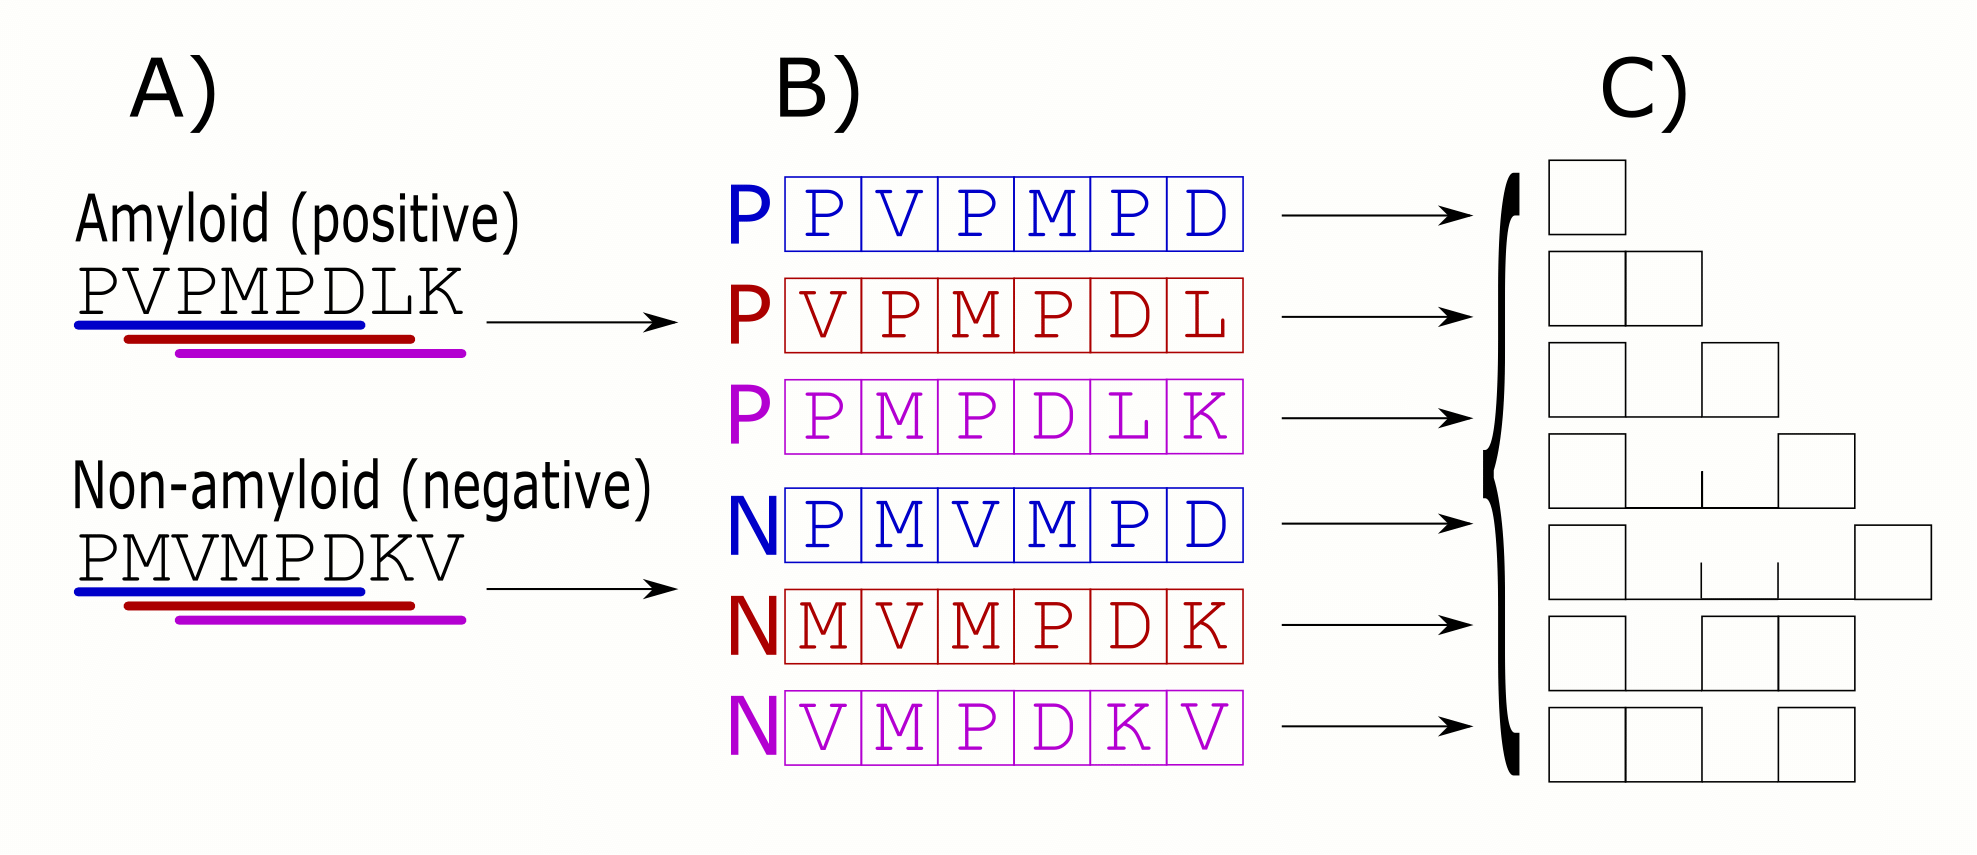
\includegraphics[width=\textwidth]{figures/ngram_scheme.png}}
\caption{The scheme of n-gram extraction. A) Input data - peptides with a known amyloidogenicity status. B) Each peptide sequence was divided into overlapping hexamers. The amyloidogenicity status of a source sequence was used as the amyloidogenicity status of a derived hexamer. C) From each hexamer we extracted continuous 1-, 2- and 3-grams. We selected also gapped 2-grams with the length of gap equal from 1 to 3 residues and gapped 3-grams with a single gap between the first and the second or the second and the third element of the n-gram.}\label{fig:ngram_scheme}
\end{figure*}

During the training phase, we extracted overlapping hexamers from each sequence. Each hexamer was tagged with the same etiquette (amyloid/nonamyloid) as the original peptide. For example, the sequence of length 6 residues yields only one hexamer and the sequence of 8 residues yields 3 hexamers.  Assuming that in longer amyloids only a short part of the sequence is responsible for amyloidogenicity, our method might results in many false positives in the training data set. To evade this problem, we restricted the maximum length of peptides in training data set to fifteen amino acids to easy the extraction of probable hot-spots. 

From each hexamer we extracted n-grams of the following length: 1, 2 and 3. In the case of 2- and 3-grams, we separately counted both gapped and continous n-grams. For 2-grams we counted n-grams with gaps of lengths from 1 to 3 and for 3-grams with a single gap between the first and the second or the second and the third element (see Fig.~\ref{fig:ngram_scheme}).

The inquire further the length of amyloidogenicity signal, we trained three classifiers for each encoding on the sequences of different length. We considered separately six-residue sequences, shorter of equal to ten residues and shorter or equal to fifteen residues.

All n-grams extracted from the hexamers in the training data set were filtered using QuiPT, our own implementation of permutation test with the information gain ( mutual information) as the criterion of the importance of a specific n-gram. In the next step, we used n-grams with the p-value smaller than 0.05 to build a random forest~\citep{breiman_random_2001} classifier using ranger \textbf{R} package~\citep{wright_ranger:_2015}. 

Furthemore, we repeated the procedure described above on two typical reduced alphabets of amino acids derived from the literature to check if the process of amyloidogenicity does require nonstandard groupings of amino acids. We also added the full amino acid alphabet to assess the advantages of the amino acid encoding.

\subsection{Cross-validation and selection of the best performing encoding}

The ability to correctly predict amyloidogenicity was assessed during the five-fold cross-validation. Since the data set was very heterogenous,  we repeated the cross-validation fifteen times for each classifier to obtain more precise estimates of peformance measures for each classifier. 

To evaluate if our classifiers are able to use decision rules extracted from sequences of given length to correctly classify longer or shorter sequences, we calculate performance measures separately for four ranges of lengths of sequences:  
\begin{itemize}
\item 6;  
\item 7-10;   
\item 11-15;   
\item 16-25.  
\end{itemize}
The number of sequences from the given length range was roughly comparable between folds of cross-validation.

To choose the most adequate reduced amino acid alphabet, we ranked the values of AUC (with rank 1 for the best AUC, rank 2 for the second best AUC and so on) for each range of sequence length in the testing data set. The encoding having the lowest sum of ranks from all sequence length categories was selected as the best one nd further used to develop AmyloGram, a predictor of amyloidogenicity.

\subsection{Benchmark}

We used pep424 data set~\cite{walsh_pasta_2014} to compare the performance of AmyloGram and other predictors of amyloidogenicity. Since the model of AmyloGram does not covers peptides shorter than five amino acids, we removed them from the total benchmark data set. It should not affect the comparison as only five sequences were eliminated (around 1\% of the original data set).

MCC to choose the best classifier.
How sensitivity/specificity depends on the lengths of sequences in the positive and negative training set.
Which the simplest (shortest) alphabet gives the best prediction.
Correlation matrix of Hamming distance of best n-grams.
Encoding distance.

\end{methods}

\section{Results}





\begin{figure*}[!tpb]
\centerline{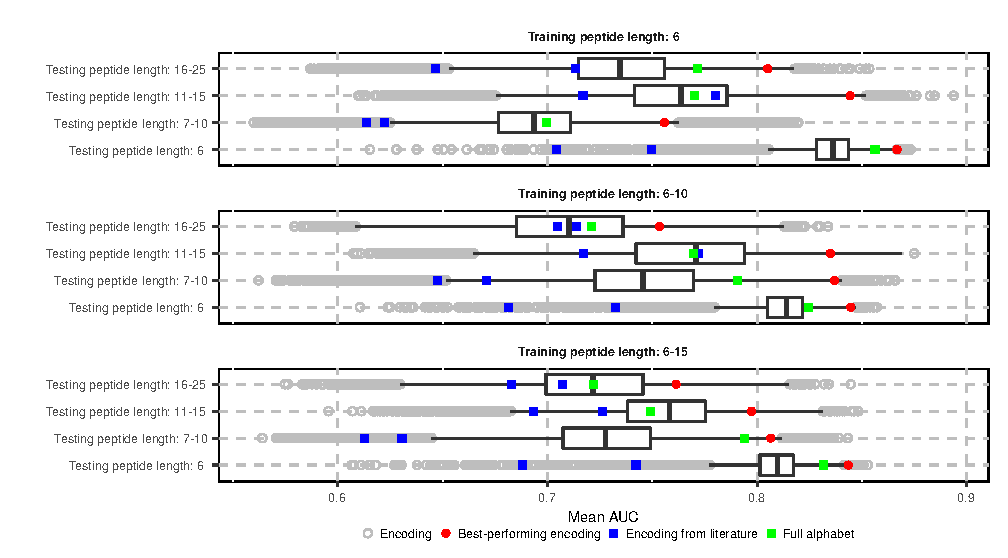
\includegraphics{figures/AUC_boxplot.eps}}
\caption{Caption, caption.}\label{fig:AUC_boxplot}
\end{figure*}



\begin{figure*}[!tpb]
\centerline{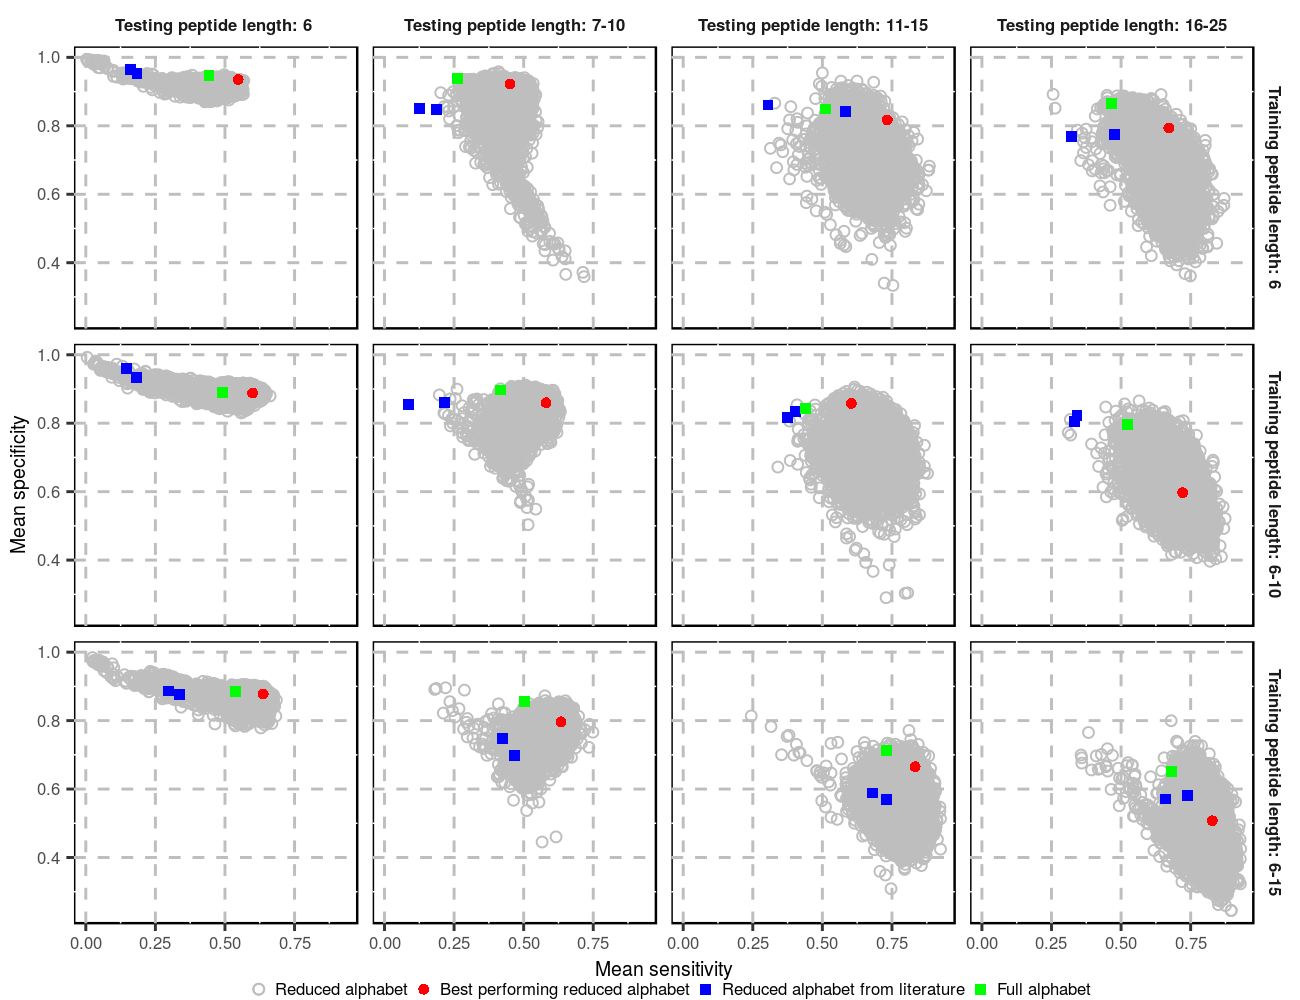
\includegraphics{figures/sesp_plot.png}}
\caption{Sensitivity and specificity of classifiers in cross-validation. Red circle: classifier employing best encoding of amino acid. Green square: classifier using full amino acid alphabet. Red square: classifiers employing encodings from literature. The classifier based on the best encoding always have good specificity and sensitivity.}\label{fig:sesp_plot}
\end{figure*}


\section{Discussion}









%%%%%%%%%%%%%%%%%%%%%%%%%%%%%%%%%%%%%%%%%%%%%%%%%%%%%%%%%%%%%%%%%%%%%%%%%%%%%%%%%%%%%
%
%     please remove the " % " symbol from \centerline{\includegraphics{fig01.eps}}
%     as it may ignore the figures.
%
%%%%%%%%%%%%%%%%%%%%%%%%%%%%%%%%%%%%%%%%%%%%%%%%%%%%%%%%%%%%%%%%%%%%%%%%%%%%%%%%%%%%%%






\section{Conclusion}



\section*{Acknowledgments}

Text Text Text Text Text Text  Text Text. 

\section*{Funding}

This research was partially funded by the KNOW Consortium.

\bibliographystyle{natbib}
%\bibliographystyle{achemnat}
%\bibliographystyle{plainnat}
%\bibliographystyle{abbrv}
%\bibliographystyle{bioinformatics}
%
%\bibliographystyle{plain}
%
\bibliography{amyloids}
\end{document}
